\label{ap:ap03}
\chapter{Linguagem R}
\section*{\textbf{A - ENUNCIADO}}
\subsection*{\textbf{1 Pesquisa com Dados de Satélite (Satellite)}}



O banco de dados consiste nos valores multiespectrais de pixels em vizinhanças 3x3 em uma imagem de satélite, e na
classificação associada ao pixel central em cada vizinhança. O objetivo é prever esta classificação, dados os valores
multiespectrais.

Um quadro de imagens do Satélite Landsat com MSS (\textit{Multispectral Scanner System}) consiste em quatro imagens
digitais da mesma cena em diferentes bandas espectrais. Duas delas estão na região visível (correspondendo
aproximadamente às regiões verde e vermelha do espectro visível) e duas no infravermelho (próximo). Cada pixel é uma
palavra binária de 8 bits, com 0 correspondendo a preto e 255 a branco. A resolução espacial de um pixel é de cerca de
80m x 80m. Cada imagem contém 2340 x 3380 desses pixels. O banco de dados é uma subárea (minúscula) de uma cena,
consistindo de 82 x 100 pixels. Cada linha de dados corresponde a uma vizinhança quadrada de pixels 3x3 completamente
contida dentro da subárea 82x100. Cada linha contém os valores de pixel nas quatro bandas espectrais (convertidas em
ASCII) de cada um dos 9 pixels na vizinhança de 3x3 e um número indicando o rótulo de classificação do pixel central.

As classes são: solo vermelho, colheita de algodão, solo cinza, solo cinza úmido, restolho de vegetação, solo cinza
muito úmido.

Os dados estão em ordem aleatória e certas linhas de dados foram removidas, portanto você não pode reconstruir a imagem
original desse conjunto de dados. Em cada linha de dados, os quatro valores espectrais para o pixel superior esquerdo
são dados primeiro, seguidos pelos quatro valores espectrais para o pixel superior central e, em seguida, para o pixel
superior direito, e assim por diante, com os pixels lidos em sequência, da esquerda para a direita e de cima para
baixo. Assim, os quatro valores espectrais para o pixel central são dados pelos atributos 17, 18, 19 e 20. Se você
quiser, pode usar apenas esses quatro atributos, ignorando os outros. Isso evita o problema que surge quando uma
vizinhança 3x3 atravessa um limite.

O banco de dados se encontra no pacote \textbf{mlbench} e é completo (não possui dados faltantes).
\newpage
Tarefas:

\begin{enumerate}[series=listWWNumxxii,label=\arabic*.,ref=\arabic*]
\item Carregue a base de dados Satellite
\item Crie partições contendo 80\% para treino e 20\% para teste
\item Treine modelos RandomForest, SVM e RNA para predição destes dados. 
\item Escolha o melhor modelo com base em suas matrizes de confusão. 
\item Indique qual modelo dá o melhor o resultado e a métrica utilizada
\end{enumerate}




\subsection*{\textbf{2 Estimativa de Volumes de Árvores}}



\textcolor{black}{Modelos de aprendizado de máquina são bastante usados na área da engenharia florestal (mensuração
florestal) para, por exemplo, estimar o volume de madeira de árvores sem ser necessário abatê-las.}

\textcolor{black}{O processo é feito pela coleta de dados (dados observados) através do abate de algumas árvores, onde
sua altura, diâmetro na altura do peito (dap), etc, são medidos de forma exata. Com estes dados, treina-se um modelo de
AM que pode estimar o volume de outras árvores da população.}

\textcolor{black}{Os modelos, chamados alométricos, são usados na área há muitos anos e são baseados em regressão
(linear ou não) para encontrar uma equação que descreve os dados. Por exemplo, o modelo de Spurr é dado por:}



{\centering
\textbf{\textcolor{black}{Volume = b0 + b1 *
dap}}\textbf{\textcolor{black}{\textsuperscript{2}}}\textbf{\textcolor{black}{ * Ht}}
\par}



\textcolor{black}{Onde dap é o diâmetro na altura do peito (1,3metros), Ht é a altura total. Tem-se vários modelos
alométricos, cada um com uma determinada característica, parâmetros, etc. Um modelo de regressão envolve aplicar os
dados observados e encontrar b0 e b1 no modelo apresentado, gerando assim uma equação que pode ser usada para prever o
volume de outras árvores.}

\textcolor{black}{Dado o arquivo }\textbf{\textcolor{black}{Volumes.csv}}\textcolor{black}{, que contém os dados de
observação, escolha um modelo de aprendizado de máquina com a melhor estimativa, a partir da estatística de
correlação.}



\textcolor{black}{Tarefas}

\begin{enumerate}[series=listWWNumxx,label=\arabic*.,ref=\arabic*]
\item \textcolor{black}{Carregar o arquivo Volumes.csv (http://www.razer.net.br/datasets/Volumes.csv)}
\item \textcolor{black}{Eliminar a coluna NR, que só apresenta um número sequencial}
\item \textcolor{black}{Criar partição de dados: treinamento 80\%, teste 20\%}
\item \textcolor{black}{Usando o pacote {\textquotedbl}caret{\textquotedbl}, treinar os modelos: Random Forest (rf), SVM
(svmRadial), Redes Neurais (neuralnet) e o modelo alométrico de SPURR}
\end{enumerate}

\begin{itemize}
\item \textcolor{black}{O modelo alométrico é dado por: Volume = b0 + b1 *
dap}\textcolor{black}{\textsuperscript{2}}\textcolor{black}{ * Ht}
\end{itemize}


\foreignlanguage{english}{\textbf{\textcolor{black}{alom {\textless}- nls(VOL \textasciitilde{} b0 + b1*DAP*DAP*HT, dados,
start=list(b0=0.5, b1=0.5)}}}\foreignlanguage{english}{\textcolor{black}{)}}



\begin{enumerate}[resume*=listWWNumxx,start=5]
\item \textcolor{black}{Efetue as predições nos dados de teste}
\item \textcolor{black}{Crie suas próprias funções (UDF) e calcule as seguintes métricas entre a predição e os dados
observados}
\end{enumerate}


\textbf{Coeficiente de determinação: }$R^2$

\begin{center}
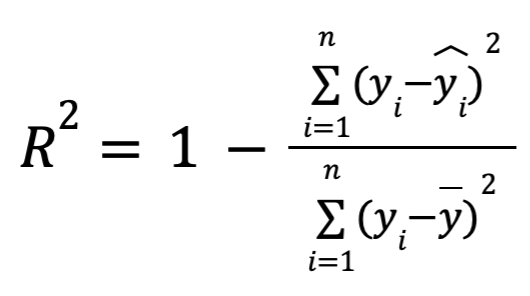
\includegraphics[width=5.191cm,height=2.9cm]{apendices/fig/IAA003_1.png} 
\end{center}

\textcolor{black}{onde } $y_i$ \textcolor{black}{\ é o valor observado, } $\widehat {y_i}$ \textcolor{black}{\ é o valor
predito e } $\overline y$ \textcolor{black}{\ é a média dos valores } $y_i$ \textcolor{black}{\ observados. Quanto mais
perto de 1 melhor é o modelo;}



\begin{itemize}
\item \textcolor{black}{Erro padrão da estimativa: S}\textcolor{black}{\textsubscript{yx}}
\end{itemize}

\begin{center}
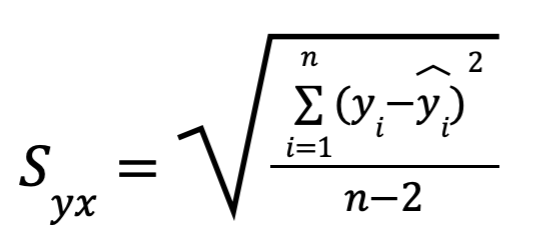
\includegraphics[width=5.117cm,height=2.32cm]{apendices/fig/IAA003_2.png} 
\end{center}

\textcolor{black}{esta métrica indica erro, portanto quanto mais perto de 0 melhor é o modelo;}



\begin{itemize}
\item \textcolor{black}{Syx\%}
\end{itemize}
\begin{center}
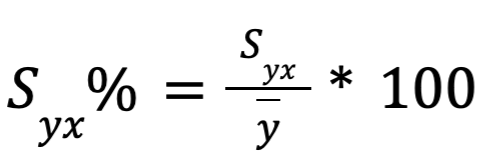
\includegraphics[width=3.688cm,height=1.235cm]{apendices/fig/IAA003_3.png}
\end{center}


\textcolor{black}{esta métrica indica porcentagem de erro, portanto quanto mais perto de 0 melhor é o modelo;}



\begin{enumerate}[resume*=listWWNumxx,start=7]
\item \textcolor{black}{Escolha o melhor modelo.}
\end{enumerate}

%%%%%%%%%%%%%%%%%%%%%%%%%%%%%%%%%%%%%%%%%%%%%%%%%%%%%%%%%%%%%%%%%%%%%%%%%%%%%%%%%%%%%%%%%%%%%
\section*{\textbf{B - RESOLUÇÃO}}

\subsection*{\textbf{1 Pesquisa com Dados de Satélite (Satellite)}}
\begin{adjustwidth}{1em}{}
\textbf{1. Carregue a base de dados Satellite}
\end{adjustwidth}
\begin{lstlisting}[language=R, style=input]
install.packages("e1071")
install.packages("randomForest")
install.packages("kernlab")
install.packages("mlbench")
install.packages("caret")
install.packages("RSNNS")

sink("./output.txt", append = T)

library(mlbench)
library(caret)
library(RSNNS)

data("Satellite")
df <- Satellite[,17:20]
df$classes <- Satellite$classes
\end{lstlisting}

\begin{adjustwidth}{1em}{}
\textbf{2. Crie partições contendo 80\% para treino e 20\% para teste}
\end{adjustwidth}
\begin{lstlisting}[language=R, style=input]
set.seed(7)
indices <- createDataPartition(df$classes, p=0.8, list=FALSE)
treino <- df[indices, ]
teste <- df[-indices, ]
\end{lstlisting}

\begin{adjustwidth}{1em}{}
\textbf{3. Treine modelos RandomForest, SVM e RNA para predição destes dados. }
\end{adjustwidth}
\begin{lstlisting}[language=R, style=input]
print(">> Iniciando treinamento rf...")
rf <- caret::train(classes~., data=treino, method="rf")
predicoes.rf <- predict(rf, teste)
confusion.rf <- caret::confusionMatrix(predicoes.rf, teste$classes)

print(">> Iniciando treinamento svm...")
svm <- caret::train(classes~., data=treino, method="svmRadial")
predicoes.svm <- predict(svm, teste)
confusion.svm <- caret::confusionMatrix(predicoes.svm, teste$classes)

print(">> Iniciando treinamento rna...")
rna <- caret::train(classes~., data=treino, method="nnet")
predicoes.rna <- predict(rna, teste)
confusion.rna <- caret::confusionMatrix(predicoes.rna, teste$classes)
\end{lstlisting}

\begin{adjustwidth}{1em}{}
\textbf{4. Escolha o melhor modelo com base em suas matrizes de confusão. }
\end{adjustwidth}
\begin{lstlisting}[language=R, style=input]
print(">> Iniciando Análises de Matrizes de Confusão...")
print(confusion.rf) #acuracia = 84%
print(confusion.svm) #acuracia = 87%
print(confusion.rna) #acuracia = 80%
\end{lstlisting}

\begin{adjustwidth}{1em}{}
\textbf{5. Indique qual modelo dá o melhor o resultado e a métrica utilizada}
\end{adjustwidth}
A métrica escolhida para comparação é a acurácia. A acurácia dos modelos são:
\begin{itemize}
    \item RandomForest: 84\%
    \item SVM: 87\%
    \item RNA: 80\%
\end{itemize}

O modelo de melhor acurácia é o SVM com 87\%.



\subsection*{\textbf{2 Estimativa de Volumes de Árvores}}
\begin{adjustwidth}{1em}{}
\textbf{1. Carregar o arquivo Volumes.csv (http://www.razer.net.br/datasets/Volumes.csv)}
\end{adjustwidth}
\begin{lstlisting}[language=R, style=input]
install.packages("mlbench")
install.packages("caret")
install.packages("RSNNS")
install.packages("kernlab")
install.packages("randomForest")

sink("./output.txt", append = T)

library(mlbench)
library(caret)
library(RSNNS)

# load dataset
df <- read.csv("./Volumes.csv", header=TRUE, sep=";")
\end{lstlisting}

\begin{adjustwidth}{1em}{}
\textbf{2. Eliminar a coluna NR, que só apresenta um número sequencial}
\end{adjustwidth}
\begin{lstlisting}[language=R, style=input]
df$DAP <- as.numeric(sub(",", ".", df$DAP, fixed = TRUE))
df$HT <- as.numeric(sub(",", ".", df$HT, fixed = TRUE))
df$HP <- as.numeric(sub(",", ".", df$HP, fixed = TRUE))
df$VOL <- as.numeric(sub(",", ".", df$VOL, fixed = TRUE))
df$NR <- NULL
summary(df)

set.seed(7)
\end{lstlisting}

\begin{adjustwidth}{1em}{}
\textbf{3. Criar partição de dados: treinamento 80\%, teste 20\%}
\end{adjustwidth}
\begin{lstlisting}[language=R, style=input]
df[c(1, 2, 3)] <- lapply(df[c(1, 2, 3)], function(x) c(scale(x)))

indices <- createDataPartition(df$VOL, p=0.80, list=FALSE)
traindf <- df[indices,]
testdf <- df[-indices,]

str(df)
\end{lstlisting}

\begin{adjustwidth}{1em}{}
\textbf{4. Usando o pacote {\textquotedbl}caret{\textquotedbl}, treinar os modelos: Random Forest (rf), SVM
(svmRadial), Redes Neurais (neuralnet) e o modelo alométrico de SPURR}
\end{adjustwidth}
\begin{lstlisting}[language=R, style=input]
# modelo alométrico de SPURR

alom <- nls(VOL ~ b0 + b1 * DAP * DAP * HT, traindf, start=list(b0=0.5, b1=0.5))
summary(alom)
str(alom)

predictalom <- predict(alom, testdf)
print(predictalom)

train_control <- trainControl(method = "cv", number = 10)

rf <- caret::train(VOL~., data=traindf, method="rf", trainControl=trainControl)

svm <- caret::train(VOL~., data=traindf, method="svmRadial", trainControl=trainControl)

rna <- caret::train(VOL~., data=traindf, method="nnet", trainControl=trainControl)
\end{lstlisting}

\begin{adjustwidth}{1em}{}
\textbf{5. Efetue as predições nos dados de teste}
\end{adjustwidth}
\begin{lstlisting}[language=R, style=input]
predictionsrf <- predict(rf, testdf)
predictionssvm <- predict(svm, testdf)
predictionsrna <- predict(rna, testdf)
\end{lstlisting}

\begin{adjustwidth}{1em}{}
\textbf{6. Crie suas próprias funções (UDF) e calcule as seguintes métricas entre a predição e os dados
observados}
\end{adjustwidth}
\begin{lstlisting}[language=R, style=input]
RSQUARE = function(y_actual,y_predict){
  cor(y_actual,y_predict)^2
}

LR_R = RSQUARE(testdf[,4], predictionsrf)
LR_R = RSQUARE(testdf[,4], predictionssvm)
LR_R = RSQUARE(testdf[,4], predictionsrna)
LR_R = RSQUARE(testdf[,4], predictalom)

syx <- function(vol, pred) {
  residual <- vol - pred
  sse <- sum(residual^2)
  n <- length(vol) - 2
  syx <- sqrt(sse / n)
  return(syx)
}

syx_r <- syx(testdf[,4], predictionsrf)
syx_r <- syx(testdf[,4], predictionssvm)
syx_r <- syx(testdf[,4], predictionsrna)
syx_r <- syx(testdf[,4], predictalom)

syx_percentual <- function(vol, pred) {
  syx_v <- syx(vol, pred)
  media_dados <- mean(vol)
  syx_percentual <- (syx_v / media_dados) * 100
  return(syx_percentual)
}

syxp_r <- syx_percentual(testdf[,4], predictionsrf)
syxp_r <- syx_percentual(testdf[,4], predictionssvm)
syxp_r <- syx_percentual(testdf[,4], predictionsrna)
syxp_r <- syx_percentual(testdf[,4], predictalom)
\end{lstlisting}

\begin{adjustwidth}{1em}{}
\textbf{7. Escolha o melhor modelo.}
\end{adjustwidth}

Três métricas foram calculadas para os modelos. São elas, Coeficiente de determinação R2, Erro padrão da estimativa Syx, e porcentagem de Syx. A seguir os valores obtivos pelas métricas em cada um dos modelos.\\

\begin{adjustwidth}{1.5em}{}
\textbf{R2} (Quanto mais perto de 1 melhor)
\end{adjustwidth}
\begin{itemize}
    \item \colorbox{LimeGreen}{RandomForest: 0.8589349}
    \item SVM: 0.856365
    \item NNET: NA
    \item SSPUR: 0.8546826
\end{itemize}

\begin{adjustwidth}{1.5em}{}
\textbf{SYX} (Quanto mais perto de 0 melhor)
\end{adjustwidth}
\begin{itemize}
    \item \colorbox{LimeGreen}{RandomForest: 0.1445527}
    \item SVM: 0.1470481
    \item NNET: 0.49606
    \item SSPUR: 0.1574296
\end{itemize}

\begin{adjustwidth}{1.5em}{}
\textbf{SYX\%} (Quanto mais perto de 0 melhor)
\end{adjustwidth}
\begin{itemize}
    \item \colorbox{LimeGreen}{RandomForest: 11.07658\%}
    \item SVM: 11.2678\%
    \item NNET: 38.01139\%
    \item SSPUR: 12.0633\%
\end{itemize}

%%%%%%%%%%%%%%%%
Como forma de melhorar os resultados, tentamos fazer a normalização dos dados como etapa de pré-processamento. Essa etapa de ``dimensionamento'' assegura que os dados de todas as colunas estejam dentro do mesmo intervalo de valores, [-2,2]. Isso evita que a rede possa acabar ``perdendo'' \textit{features} com valores muito pequenos, e que seriam relevantes durante o treinamento, em seus cálculos, privilegiando \textit{features} com valores muito mais altos.

Após realizar a normalização e padronização dos dados, com a aplicação da função \textbf{scale} nas colunas DAP, HP e HT da base de dados, pudemos observar uma leve melhora em algumas métricas, mas principalmente, conseguimos um resultado muito mais expressivo para o treinamento da RNA.

Ao mesmo tempo, o resultado do modelo alométrico de SPURR teve uma grande piora na métrica R2, provavelmente porque ele funciona através de uma aproximação à função de volume e a mudança dos valores interfira nos cálculos. 

%%%%%%%%%%%%%%%%

\begin{adjustwidth}{1.5em}{}
\textbf{R2}
\end{adjustwidth}
\begin{itemize}
    \item \colorbox{LimeGreen}{RandomForest: 0.8601537} \FancyUpArrow
    \item SVM: 0.856365
    \item NNET: 0.4843006 \FancyUpArrow 
    \item SSPUR: 0.5317544 \FancyUpDown
\end{itemize}

\begin{adjustwidth}{1.5em}{}
\textbf{SYX}
\end{adjustwidth}
\begin{itemize}
    \item \colorbox{LimeGreen}{RandomForest: 0.1438805} \FancyUpDown
    \item SVM: 0.1470481
    \item NNET: 0.4960265 \FancyUpDown
    \item SSPUR: 0.3854788 \FancyUpArrow 
\end{itemize}

\begin{adjustwidth}{1.5em}{}
\textbf{SYX\%}
\end{adjustwidth}
\begin{itemize}
    \item \colorbox{LimeGreen}{RandomForest: 11.02507\%} \FancyUpDown
    \item SVM: 11.2678\%
    \item NNET: 38.00883\% \FancyUpDown
    \item SSPUR: 29.53794\% \FancyUpArrow 
\end{itemize}


Escolhemos o modelo RandomForest como melhor por ter se saído ligeiramente melhor em todas as métricas calculadas.